\documentclass{article}
\usepackage{times}
\documentclass{article}
\usepackage{amssymb}
\usepackage{amsmath}
\usepackage{graphicx} % Required for inserting images
\usepackage[a4paper, total={7in, 10in}]{geometry}

\title{Lista 2 - MAC0320}
\author{Paulo Henrique Albuquerque, NUSP $=12542251$ }
\date{}

\begin{document}

\maketitle

\textbf{E6.} 
\vspace{5mm}

\textbf{Solução.} 



\end{document}




\title{Sistemas de arquivos \\ {\large \color{red}Notas do capítulo 5}}

\newcommand\unix{{\color{red}UNIX} }
\newcommand\msdos{{\color{yellow}MS-DOS} }
\newcommand\winxp{{\color{blue}Windows XP} }
\newcommand\winnoveoito{{\color{pink}Windows 98} }
\newcommand\winnovecinco{{\color{green}Windows 95} }

\begin{document}

\maketitle

\section{Introdução aos arquivos}
Os três requisitos para armazenamento de informação a longo prazo são:

\begin{itemize}
  \item deve ser possível armazenar uma grande quantidade de informação.
  \item a informação deve sobreviver à terminação do processo que a usa. 
  \item múltiplos processos devem ser capazes de acessar a informação de forma concorrente.
\end{itemize}

A solução usual para todos esses problemas é armazenar informação em discos em unidades chamadas \textbf{arquivos}. A informação presente nessas unidades precisa ser \textbf{persistente}, ou seja, não deve ser afetada pela criação ou terminação de processos.

Arquivos são gerenciados pelo sistema operacional. A parte do SO responsável por esse gerenciamento é conhecido como o \textbf{sistema de arquivos}.

\subsection{Arquivos}

\subsubsection{Nomes de arquivos}
Arquivos são abstrações. Eles são uma forma de armazenar informação em disco para ser lida depois. Isso deve ser feito de forma que o usuário não precise se preocupar com os detalhes de como a informação é armazenada e como discos funcionam. Uma das características mais importantes de um \textit{mecanismo de abstração} é como os objetos são nomeados. Examinemos como arquivos são nomeados nos diferentes sistemas de arquivos.
No sistema \unix, há distinção entre letras maíusculas e minúsculas, \msdos não faz essa distinção.

O sistema \winxp tem um sistema nativo, o New Technology File System (NTFS) que suporta nomes de arquivos em Unicode. 

Em alguns sistemas, como \unix, extenções não são forçadas. O Windows é bastante ciente das extensões dos arquivos e atribui significado para as diferentes extensões. Algo estranho nesse sistema é que, apesar das extensões serem importantes, elas são escondidas por padrão. Isso pode ser alterado pelo usuário.

\subsubsection{Estrutura dos arquivos}
Há três formas comuns para estruturar arquivos:
\begin{itemize}

    \item arquivo como uma simples sequência de bytes. Esse é o jeito \unix e \winnoveoito. O sistema não se importa com o que está no arquivo, tudo que vê são bytes. Qualquer significado é imposto por programas de usuário.  
  \item arquivo como sequência de registros de tamanhos fixos. Cada registro tem um estrutura interna. As operações de leitura e escrita atuam sobre registros.
  \item arquivo como um árvore de registros. Cada registro tem um chave, que é usada para buscas rápidas. É amplamente utilizado em mainframes ainda utilizados em grandes centros de processamento de dados.

\end{itemize}

\begin{figure}[h!]
  \begin{center}
    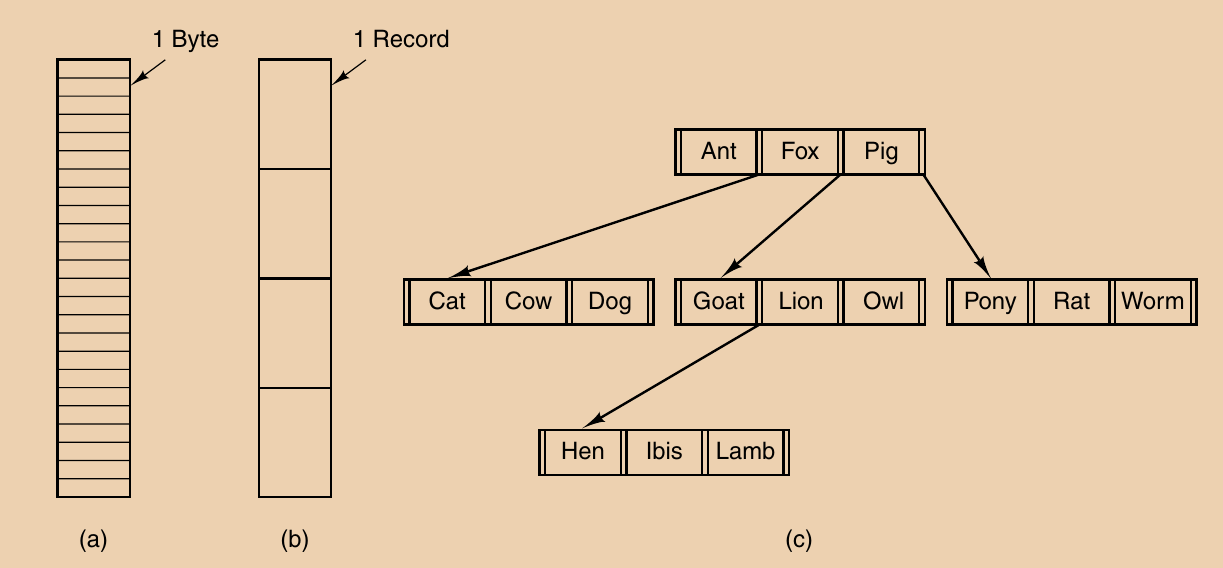
\includegraphics[width=0.45\textwidth]{img/5-2.png}
  \end{center}
  \caption{Tipos de estruturas para arquivos}
  \label{fig:}
\end{figure}

\subsubsection{Tipos de arquivos}
Há vários tipos de arquivos definidos em diferentes SOs. O \unix define \textbf{arquivos regulares e diretórios}, além de definir arquivos especiais, de bloco e de caracteres. No \winxp há arquivos de \textbf{metadados}.


\textbf{Arquivos regulares} contém informações de usuário. \textbf{Diretórios} são arquivos de sistema que mantêm a estrutura do sistema de arquivos. \textbf{Arquivos de caracteres} estão relacionados a dispositivos I/O. \textbf{Arquivos de bloco} são usados para modelar discos. Estamos interessados aqui em arquivos regulares e de diretórios, principalmente.

Em geral, arquivos regulares são arquivos texto (ASCII) ou arquivos binários. Arquivos binários têm uma esrtutura interna conhecida pelos programas que os usam. 
Um exemplo de arquivo binário é um arquivo executável do \unix ou um arquivo "archive", também do \unix. Eles são mostrados na figura abaixo.

\begin{figure}[h]
  \begin{center}
    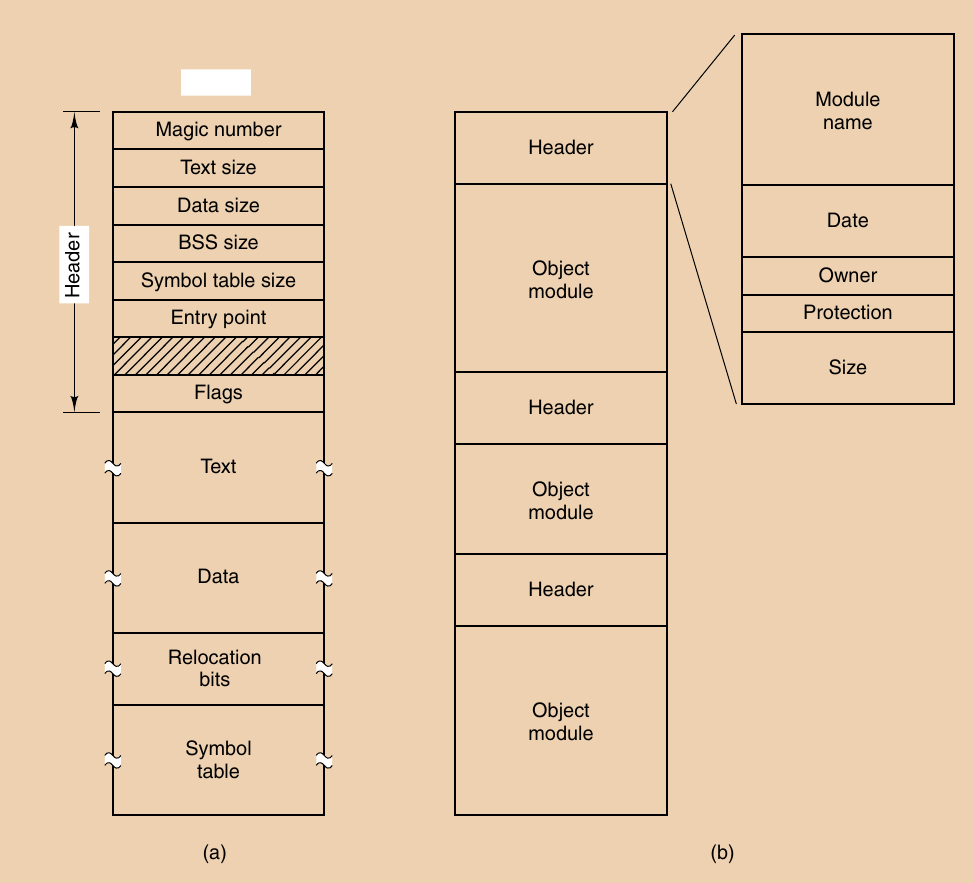
\includegraphics[width=0.45\textwidth]{img/5-3.png}
  \end{center}
  \caption{}
  \label{fig:}
\end{figure}

Apesar do SO enxergar um arquivo executável apenas como uma sequência de bytes, ele somente irá executá-lo se o arquivo tiver um formato adequado. Por exemplo, na seção "header" de um executável do \unix, o campo \textbf{magic number} identifica o arquivo como executável: arquivos que não têm essa flag ativada não serão executados pelo SO. Seguido do header, há o segmento de texto e de dados do programa. Eles são carregados na memória.

\subsubsection{Acesso de arquivos}

Há dois tipos comuns de acesso a arquivos, sequencial e aleatório. Sistemas antigos só forneciam o primeiro. Nesse tipo de acesso, um processo deve ler os bytes de um arquivo em ordem. Quando discos são utilizados para armazenar arquivos, é possível ler bytes fora de ordem. Arquivos que podem ser acessados fora de ordem são chamados de \textbf{arquivos de acesso aleatório}. Eles são necessários para várias aplicações. Por exemplo, se um cliente de uma companhia aérea deseja reservear uma vaga em um voo, o programa que faz a reserva deve ser capaz de acessar o arquivo de reservas desse vôo sem ter que ler os arquivos de milhares de outros vôos. 

Há dois métodos para especificar onde começar a ler o arquivo. No primeiro, toda operação \verb|read| dá a posição no arquivo onde começa a leitura. No segundo, a chamada \verb|seek| é feita para configurar a posição corrente de leitura. Depois dessa chamada, o arquivo pode ser lido sequencialmente. 

Sistemas operacionais modernos consideram todos os arquivos como de acesso aleatório.

\subsubsection{Atributos de arquivos}

Todo arquivo tem um nome e seus dados. Em adição a isso, todos sistemas operacionais associam outras informações a cada arquivo, por exemplo, a data de criação do arquivo. Essas informações adicionais são chamadas de \textbf{atributos} do arquivo. Algumas pessoas chamam de \textbf{meta dados}. A lista de atributos depende da implemnetação de cada sistema operacional.

Alguns atributos possíveis são mostrados abaixo.

\begin{figure}[h]
  \begin{center}
    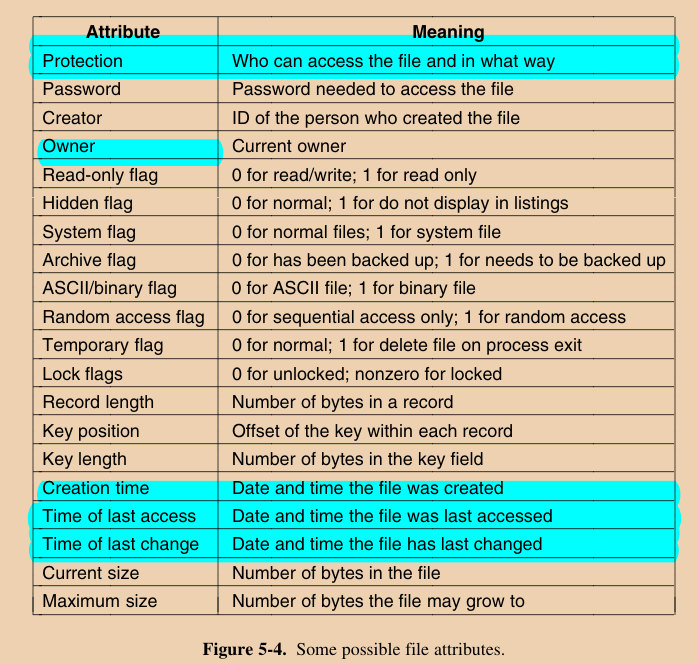
\includegraphics[width=0.45\textwidth]{img/5-4.png}
  \end{center}
  \caption{}
  \label{fig:}
\end{figure}

Os vários atributos de "tempo" marcam quando o arquivo foi criado, tempo do último acesso e tempo de última modificação. Esses atributos são úteis para vários programas. Por exemplo, um código fonte modificado desde a última compilação deve ser compilado novamente.

\subsection{Operações}

Abaixo listamos as operações possíveis em arquivos, juto com uma breve descrição.

\begin{itemize}
  \item Create. O arquivo é criado sem nenhum dado. O objetivo dessa call é avisar ao SO que um arquivo foi criado e assim ele pode configurar alguns atributos.
  \item Delete. Deleta o arquivo para liberar espaço no disco.
  \item Open. Antes de usar um arquivo, ele precisa ser aberto. O propósito dessa chamada é permitir que o SO traga os atributos e lista de endereços de blocos de discos do arquivo para memória para acessos futuros rápidos.
  \item Close. O arquivo é liberado para liberar memória.
  \item Read. Lê dados do arquivo. A chamada deve especificar a quantidade de bytes que deseja ler e um buffer para armazená-los.
  \item Write. Escreve no arquivo.
  \item Append. Escreve no final do arquivo.
  \item Seek. Reposiciona o ponteiro de arquivo para leitura ou escrita. 
  \item Get attributes.
  \item Set attributes.
  \item Rename.
  \item Lock. Proibe acesso simultâneo por diferentes processos.
\end{itemize}

\section{Diretórios}
São utilizados para manter a estrutura do sistema de arquivos. Em muitos sistemas, são arquivos.

\subsection{Diretórios simples}
Um diretório simples contém um número de entradas, uma por arquivo.

Quando um arquivo é aberto, o SO procura seu diretório até achar o nome do arquivo a ser aberto. Após encontrar, extrai os atributos e endereços de discos da entrada do diretório ou da estrutura de dados apontada por ela, e coloca esses dados na memória. Todas referências futuras ao arquivo são feitas usando essas informações na memória.

O número de diretórios varia de sistema para sistema. A forma mais simples é um único diretório contendo todos os arquivos de todos os usuários. Isso é problemático em situações em que múltiplos usuários usam nomes de arquivos iguais: nesse cenário, o sistema não consegue distinguir os dois arquivos quando uma chamada Open é feita, por exemplo. 

Uma possível solução para isso é utilizar diferentes diretórios para diferentes usuários. Isso permite nomes iguais de arquivos para diferentes usuários.

Outra melhora possível é permitir que um mesmo usuário tenha vários diretórios, para propósitos de organização. Isso é uma \textbf{hierarquia geral}, ou seja, uma árvore de diretórios. Veja a figura abaixo.

\begin{figure}[h]
  \begin{center}
    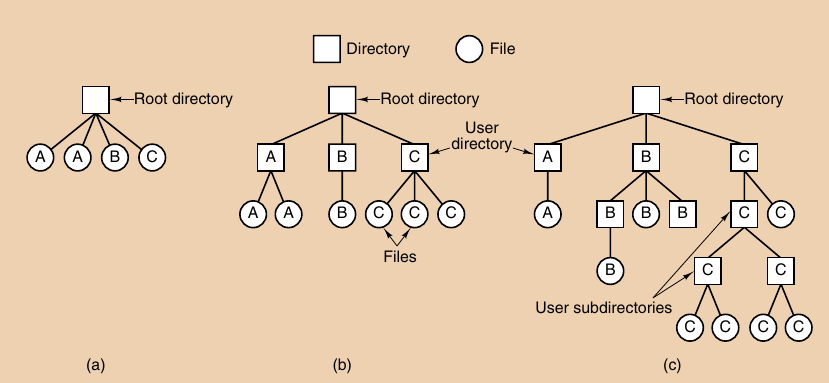
\includegraphics[width=0.45\textwidth]{img/5-6.png}
  \end{center}
  \caption{}
  \label{fig:}
\end{figure}

Pelo grande poder de organização oferecido por essa última estrutura de diretório, quase todos sistemas de arquivos modernos a utilizam.

\subsection{Caminhos}

Dois métodos são utilizados para especificar o caminho de arquivos na árvore: \textbf{caminhos absolutos} e \textbf{caminhos relativos}. Caminhos absolutos começam com "/" (No \unix) e consistem de um caminho a partir da raiz da árvore de diretórios (root). Caminhos relativos são caminhos relativos ao diretório corrente (working directory "pwd"). O diretório corrente é um conceito utilizado para que processos possam especificar a partir de onde caminhos relativos devem começar. Cada processo tem seu próprio diretório corrente.

No \unix e na maioria dos sistemas modernos, cada diretório faz referência a si mesmo com "." e ao seu pai na árvore com "..".

\subsection{Operações em diretórios}

\begin{itemize}
  \item Create. Um diretório é criado vazio com exceção do "." e "..".
  \item Delete. Somente diretórios vazios podem ser deletados do sistema de arquivos. Um diretório apenas com "." e ".." é considerado vazio.
  \item Opendir.
  \item Closedir.
  \item Readdir.
  \item Rename.
  \item Link.
  \item Unlink.
\end{itemize}

\section{Implementação de Sistemas de Arquivos}

Agora analisemos o lado do implementador de sistemas de arquivos. Eles estão interessados em como arquivos e diretórios são armazenados, como espaço de disco é gerenciado e como fazer tudo funcionar eficientemente.

\subsection{Layout}
Sistemas de arquivos são geralmente armazenados em discos.

A maioria dos discos podem ser divididos em partições, com sistemas de arquivos independentes. O setor 0 do disco é chamado de \textbf{MBR} (Master Boot Record) e é usado para o boot. O final do MBR contém a tabela de partições, que dá os começos e finais de cada partição. Uma partição é marcada como ativa. Quando o computador é iniciado, a BIOS lê e executa o código no MBR. A primeira coisa que o programa no MBR faz é localizar a partição ativa, lê seu primeiro bloco, chamado \textbf{bloco de boot} e o executa. Esse código carrega o sistema operacional contido naquela partição. Toda partição contém um bloco de boot, mesmo que não contenha nenhuma SO. A descrição acima deve ser respeitada para todo hardware que utiliza BIOS para inicializar sistemas operacionais. 
 
Vale ressaltar que alguns sistemas não exigem uma partição ativa: eles fornecem um menu para que o usuário escolha uma partição para boot. 

O layout de partição varia de sistema para sistema. Para sistemas baseados no \unix, o sistema de arquivo contém alguns dos itens mostrados na figura abaixo. Abaixo mostramos uma possível ordem de seções na partição.

\begin{figure}[h]
  \begin{center}
    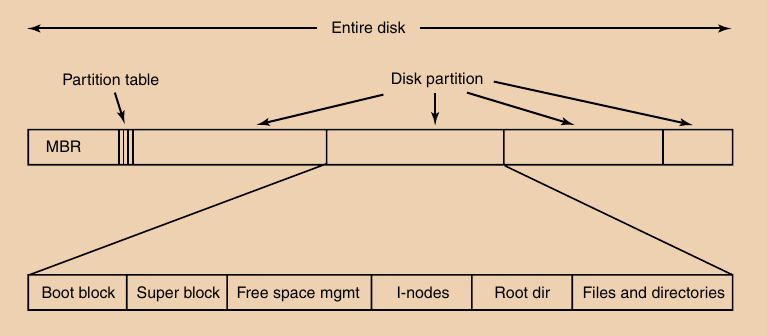
\includegraphics[width=0.45\textwidth]{img/5-8.png}
  \end{center}
  \caption{}
  \label{fig:}
\end{figure}


\begin{itemize}
  \item 1. Superblock. Contém todos os atributos principais do sistema de arquivos e é levado para a memória quando o computador é inicializado.
  \item 2. Blocos livres.
  \item 3. I-nodes. Estrutura de dados que diz tudo sobre cada arquivo e aonde estão localizados seus blocos.
  \item 4. Diretório root.
  \item 5. Todo o restante dos arquivos e diretórios.
\end{itemize}

\subsection{Implementando arquivos}

A questão mais importante sobre implementação de arquivos é guardar os blocos correspondentes a cada arquivo.

\subsubsection{Alocação contínua}

O esquema mais simplório é armazenar cada arquivo como uma sequência contínua de blocos de disco. Isso é suficientemente simples pois basta guardamos o endereço do primeiro bloco do arquivo e a quantidade de blocos no arquivo. Esse esquema também é eficiente porque um arquivo pode ser lido apenas com um \verb|read|. Apenas um \verb|read| é necessário (para o primeiro bloco do arquivo).

Um grande problema desse esquema é que, com o tempo o disco torna-se fragmentado, e quando o disco enche, é necessário fazer uma compactação, o que é muito custoso. Outra alternativa é reutilizar blocos livres. Isso é possível mantendo uma lista de blocos livre. A princípio isso é factível. Porém, quando um novo arquivo for criado é necessário especificar o tamanho final do arquivo, o que não é possível na maioria dos cenários.

Hoje em dia, há alguns usos de alocação contínua: CD-ROM's e DVD's.

\subsubsection{Listas ligadas}

Uma segunda alternativa para armazenar arquivos é manter uma lista ligadas dos blocos utilizados por cada arquivo. A primeira palavra de cada bloco é usada como ponteiro para o próximo bloco da lista, o restante do bloco é utilizado para dados.

\begin{figure}[h]
  \begin{center}
    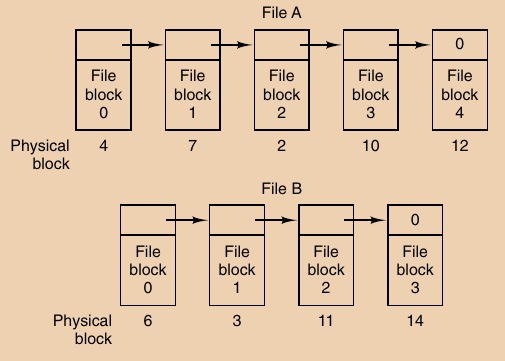
\includegraphics[width=0.45\textwidth]{img/5-9.png}
  \end{center}
  \caption{}
  \label{fig:}
\end{figure}

Todos os blocos do disco podem ser utilizados nesse esquema. Nenhum espaço é perdido devido a fragmentação. Além disso, é suficiente para a entrada no diretório desse arquivo somente armazenar o endereço para o primeiro bloco: o restante pode ser encontrado a partir daí. 

Ler um arquivo sequencialmente é fácil: para ler $n$ bytes consecutivos, são feitas $n$ leituras de blocos. Cada leitura dá um "pedaço" dos dados e o endereço do próximo bloco que deve ser lido. Já para acesso aleatório o processo é ineficiente. Para acessar o $n$-ésimo bloco, o sistema precisa ler os $n-1$ blocos anteriores, para saber qual o endereço do $n$-ésimo bloco. Outro ponto negativo desse esquema é que a quantidade de dados num bloco não é potência de dois, por causa do espaço necessário para os ponteiros. Alguns programas leêm e escrevem em blocos cujo tamanho é potência de dois. Além disso, nesse esquema é necessário concatenar informações de discos, o que gera overhead devido a cópia.

\subsubsection{Listas ligadas usando tabela em memória}

Ambas desvantagens do esquema anterior podem ser resolvidas ao colocar todas as palavras referentes ao ponteiros numa tabela em memória. Uma tabela desse tipo é chamada \textbf{FAT (File Allocation Table)}.

\begin{figure}[h]
  \begin{center}
    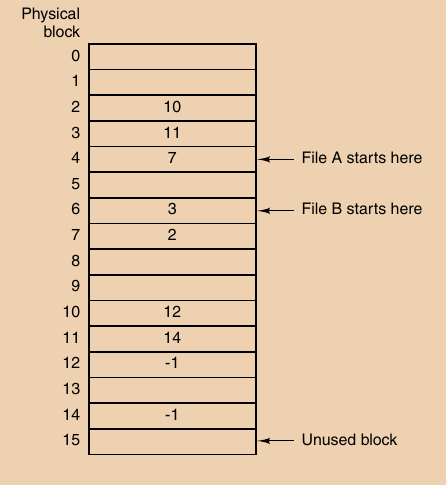
\includegraphics[width=0.45\textwidth]{img/5-10.png}
  \end{center}
  \caption{}
  \label{fig:}
\end{figure}

Usando essa organização, todo o bloco fica disponível para dados. Além disso, acesso aleatório é simples, pois podemos encontrar o endereço do bloco inicial (referente ao offset desejado) apenas utilizando as informações na memória, o que é bem mais rápido do que "seguir ponteiros" fazendo leituras no disco. As entradas de diretório dos arquivos devem guardar somente o endereço do bloco inicial.

A desvantagem principal desse método é que a tabela inteira deve estar na memória a todo tempo.

\subsubsection{I-Nodes}

O último método é associar cada arquivo a uma estrutura de dados chamada de \textbf{i-node} (\textbf{index-node}), que lista os atributos e endereços de disco dos blocos do arquivo. A grande vantagem desse esquema em relação aos esquemas anteriores é que somente o i-node do arquivo a ser aberto precisa estar na memória.

Um problema que surge com i-nodes é que cada arquivo tem uma quantidade fixa de referências à endereços de disco, mas o arquivo pode crescer indefinidamente. Nesses casos, uma solução é reservar o último endereço de disco não para um bloco de dados, e sim para um \textbf{bloco indireto} que faz referências para outros endereços de blocos. Essa ideia pode ser extendida para \textbf{blocos indiretos duplos} e \textbf{blocos indiretos triplos}, como mostrado na figura abaixo.

\begin{figure}[h]
  \begin{center}
    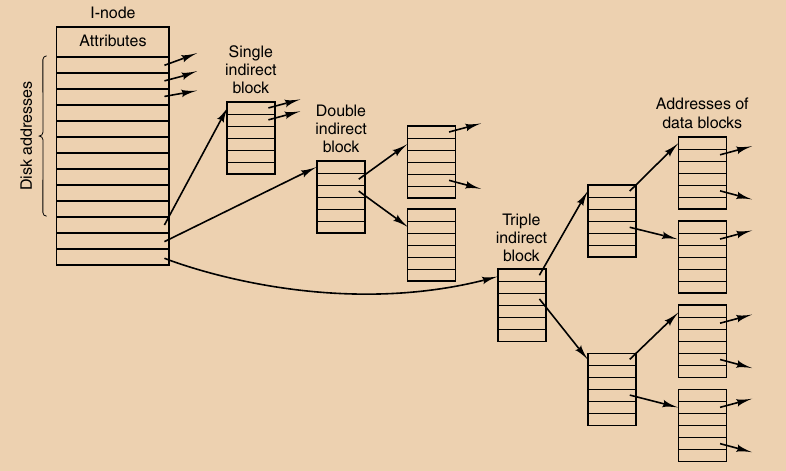
\includegraphics[width=0.45\textwidth]{img/5-11.png}
  \end{center}
  \caption{}
  \label{fig:}
\end{figure}

\subsection{Implementando diretórios}

Para que o sistema leia um arquivo ele precisa ser aberto, e para ele ser aberto ele precisa ser primeiramente achado a partir do caminho fornecido pelo usuário. O primeiro passo é localizar o diretório root. Esse diretório pode estar numa posição fixa relativa ao início de uma partição. Alternativamente, sua posição pode ser determinada \textit{a partir de outras informações}. Por exemplo, em um sistema clássico \unix, o superblock contém informação sobre o tamanho das estruturas de dados que precedem a área de dados. Ou seja, a área de "Free space mgmt" no diagrama da partição de um sistema de arquivos \unix. Então, podemos identificar o começo dos i-nodes. O primeiro i-node é o da raiz (ele é criado quando o sistema de arquivos é criado). No \winxp, a informação no setor de soot localiza a \textbf{MFT (Master File Table)}, que é usada para localizar outras partes do sistema de arquivos.

Localizada a raiz, uma busca na árvore é feita para encontrar a entrada de diretório do arquivo requerido. Ela contém as informações necessárias para acessar os blocos do arquivo. Em qualquer caso de esquema, o objetivo principal do sistema de diretórios é mapear nomes de arquivos em ASCII para as informações necessárias para localizar os dados.

Agora, surge a pergunta: onde armazenar os atributos de um arquivo? Uma possibilidade óbvia é armazenar diretamente na entrada do diretório. Nesse caso, a entrada do diretório contém o nome do arquivo, uma estrutura que armazena os atributos e um ou mais endereços de disco, que dizem onde os blocos estão. Tudo com tamanhos pré-definidos.

Para sistemas que usam i-nodes, outra possibilidade é armazenar os atributos nos próprios i-nodes. Nesse caso, a entrada do diretório de um arquivo contém somente o nome do arquivo e o número do i-node correspondente.

\subsubsection{Arquivos compartilhados}

Veja a figura abaixo, que mostra um arquivo compartilhado entre dois diretórios distintos.

\begin{figure}[h]
  \begin{center}
    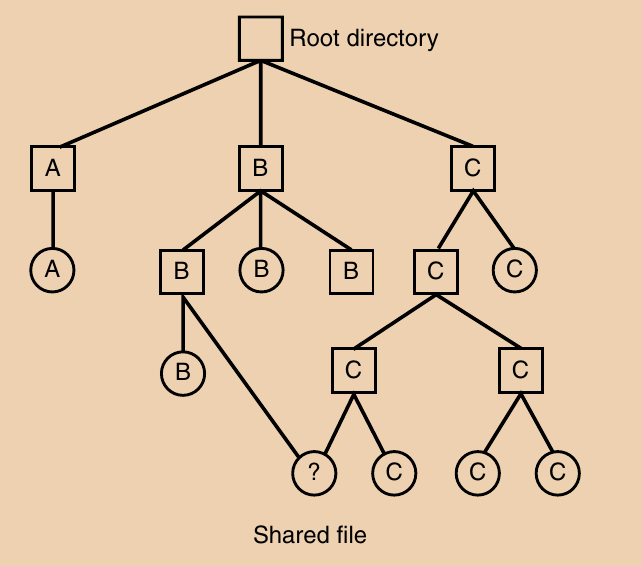
\includegraphics[width=0.45\textwidth]{img/5-12.png}
  \end{center}
  \caption{}
  \label{fig:}
\end{figure}

No \unix, o uso de i-nodes para armazenar atributos de arquivos faz com que compartilhamento de arquivos seja simples: qualquer número de diretórios pode apontar para um único i-node.

O i-node contém um campo que é incrementado quando um novo link é adicionado, e é decrementado quando um link é removido. Somente quando o contador chega a zero os dados e o i-node são deletados.

Esse tipo de link é chamado de \textbf{link físico}. Esse tipo de link tem duas "fraquezas". A primeira é que links só podem ser feitos dentro de um mesmo sistema de arquivos (partição). A outra é que a um i-node está associado somente um conjunto de atributos. Então, em uma situação em que há compartilhamento de um arquivo, o dono do arquivo pode deletar a sua entrada do diretório e outros usuários que apontam para esse arquivo ficaram impossibilitados de modificá-lo ou deletá-lo, pois os atributos dele ainda apontam o usuário original como dono do arquivo.

Há outra forma de compartilhar arquivos. Nela, cria-se um arquivo cujos "dados" é um caminho para outro arquivo. Esse tipo de link funciona através de diferentes sistemas de arquivos. Esse tipo de link é chamado de \textbf{link simbólico} em sistemas \unix, \textbf{atalho} em sistemas Windows e um \textbf{alias} no MAC OS. Links simbólicos podem ser usados em sistemas que armazenam atributos dentro da entrada do diretório. É difícil sincronizar diferentes diretórios contendo diferentes atributos para esse arquivo: uma mudança no arquivo deve afetar toda entrada de diretório apontando para esse arquivo. Mas as entradas de diretório extras não contêm os atributos desse arquivo, por isso a dificuldade. Outro problema é que quando um arquivo é deletado, links para ele se tornam orfãos.

As sutilezas desses tipos de links podem ser observadas abrindo um terminal no UNIX e testando remoções e modificações (bom exercício).

Agora, vemos algumas implementações de diretórios em diferentes sistemas.

\subsubsection{Diretórios no \winnoveoito}

O sistema de arquivos do release original do \winnovecinco era idêntico ao sistema de arquivos do \msdos, mas um novo release adicionou suporte para nomes de arquivos mais longos e arquivos maiores. Esse novo release é referido como o sistema de arquivos do \winnoveoito, apesar de ser encontrado em alguns sistemas \winnovecinco.

Há dois tipos de diretórios no \winnoveoito. O mostrado abaixo chamamos de \textbf{base entry}.

\begin{figure}[h]
  \begin{center}
    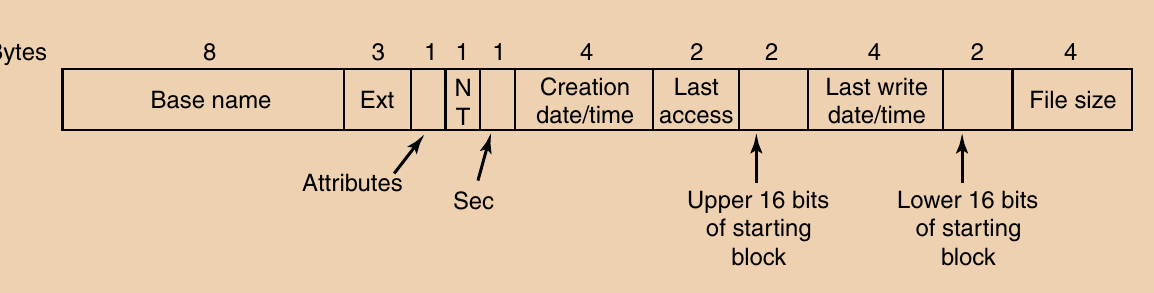
\includegraphics[width=0.45\textwidth]{img/5-13.png}
  \end{center}
  \caption{}
  \label{fig:}
\end{figure}

Essa entrada de diretório "base" contém todas as informações contidas em versões passadas do Windows e mais. O upgrade mais importante foi o aumento de bits para o campo que aponta para o primeiro bloco de 16 para 32. Isso aumentou o sistema de arquivos de $2^{16}$ blocos para $2^{32}$ blocos, o que é um aumento grande.

Essa estrutura provém apenas para o antigo estilo de nome de arquivos 8 + 3 caracteres herdado do \msdos. E nomes de arquivos longos? A resposta para esse problema enquanto mantém a retro-compatibilidade com sistemas passados é usar entradas de diretório adicionais. A figura abaixo mostra outro tipo de entrada de diretório, que pode conter até 13 caracteres de um nome de arquivo longo. Um arquivo pode estar associado a várias entradas desse tipo. Elas são colocadas antes da entrada "base" em ordem reversa. O campo "Attributes" de cada entrada de nome longo contém o valor 0xF, que é impossível para sistemas de arquivos de SO's antigos (\msdos e \winnovecinco). Então essas entradas são ignoradas em sistemas antigos. O campo "Sequence" diz ao sistema qual é a última entrada. 

Se isso parece uma confusão é porque é: prover retro-compatibilidade enquanto adiciona novas funcionalidades para um sistema novo geralmente gera uma bagunça.

\newpage

\subsubsection{Diretórios no \unix}

A estrutura tradicional de um diretório \unix é extremamete simples. Cada entrada contém um nome de arquivo e o número do seu i-node. Todas as informações adicionais do arquivo estão no i-node. 

\begin{figure}[h]
  \begin{center}
    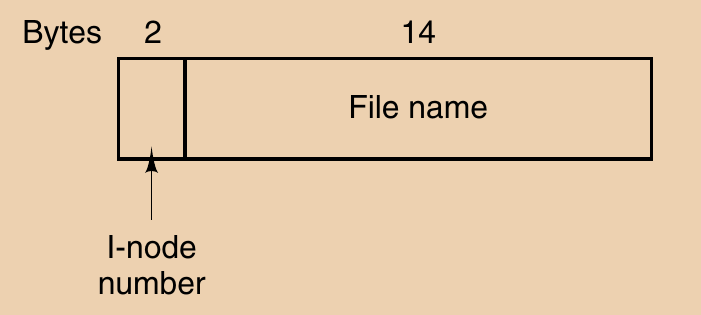
\includegraphics[width=0.3\textwidth]{img/5-15.png}
  \end{center}
  \caption{}
  \label{fig:}
\end{figure}

Quando um arquivo é aberto, o sistema deve achar os blocos do arquivo. Primeiro o sistema localiza a raiz da árvore do sistema de arquivos. Os i-nodes formam um simples array que são localizados usando as informações do superbloco. A primeira entrada do array é o i-node do root. Após localizar o i-node do root, o sistema lê o conteúdo do diretório root, que dára o i-node do próximo diretório, e assim por diante. 

\begin{figure}[h]
  \begin{center}
    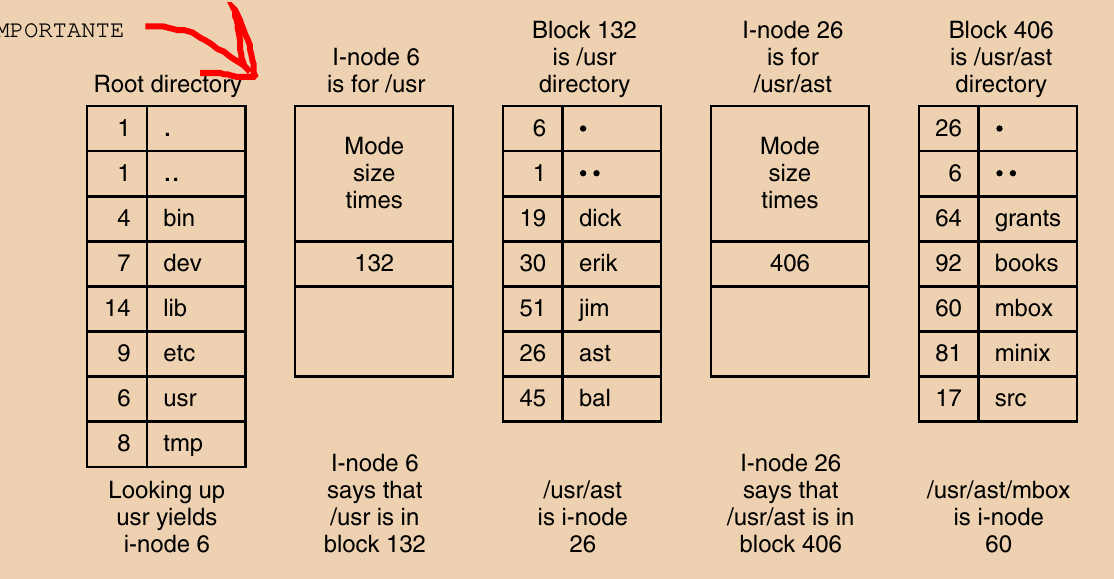
\includegraphics[width=0.45\textwidth]{img/5-16.png}
  \end{center}
  \caption{}
  \label{fig:}
\end{figure}

Caminhos relativos são localizados da mesma forma que caminhos absolutos, só que começando no diretório corrente do processo. Nenhum mecanismo especial é utilizado para tratar os diretórios "." e "..": para o sistema de arquivos, eles são só strings ASCII ordinárias e são tratadas da mesma forma que os outros nomes.

\subsubsection{Diretórios no NTFS}

O sistema \textbf{NTFS} (\textbf{New Technology File System}) da Microsoft é o sistema de arquivos padrão. Ele provém múltiplos conjuntos de caracteres ao usar Unicode para nome de arquivos. Mas usar múltiplas linguagens faz surgirem alguns problemas. Por exemplo, algumas línguas têm formas de ordenação lexicográfica distintas. A solução é ter um atributo somente para convenções de linguagem para a língua do arquivo em questão. "Mais atributos" é a solução NTFS para vários problemas. 

No \unix, um arquivo é somente uma sequência de bytes. No NTFS, um arquivo é uma coleção de atributos, e cada atributo é uma stream de bytes. A estrutura de dados básica é a \textbf{MFT} (\textbf{Master File Table}) que fornece 16 atributos, onde cada um pode ter 1 KB. Um atributo dentro da MFT pode ser um ponteiro para um arquivo adicional se necessário. 

Os dados no NTFS são armazenados em um atributo. Um arquivo NTFS pode ter mais de uma stream de dados. Múltiplas streams de dados podem ter vários usos. Por exemplo, uma imagem grande pode ter uma pequena thumbnail associada a ela, e essas duas imagens podem ser armazenadas em streams diferentes de dados. No outro extremo, NTFS pode lidar com arquivos pequenos colocando centenas de bytes no atributo header. Isso é chamado de uma \textbf{arquivo imediato} (Mullender and Tanenbaum, 1984).

\subsubsection{Gerenciamento de espaço em disco}

Arquivos são normalmente armazenados em discos. Evidentemente, gerenciamento de espaço de disco é uma grande preocupação para os implementadores de sistemas. Conforme vimos, há duas formas principais de armazenar um arquivo de $n$ bytes: usando $n$ bytes consecutivos no discos ou usando um número de blocos não necessariamente consecutivos. Armazenar de forma consecutiva tem a desvantagem de, que se um arquivo cresce, provavelmente terá de ser movido no disco, o que é bastante custoso. Por essa razão, quase todos os sistemas "cortam" o arquivo em blocos de tamanho fixado que não são adjacentes no disco.

\subsubsection{Tamanho do bloco}

Naturalmente, surge a pergunta: qual tamanho de bloco utilizar? Utilizar conhecimentos sobre a estrutura interna do disco é claramente uma forma de tomar essa decisão. Porém, isso é altamente dependente do dispositivo, o que é uma grande desvantagem. 

Um tamanho grande demais de bloco faz com que arquivos pequenos utilizem um cilindro inteiro, por exemplo. Tamanhos pequenos demais, fazem com que cada arquivo consiste em um grande número de blocos. Ler cada bloco normalmente requer um \textit{seek} e um \textit{rotational delay} o que torna a leitura de todos esses blocos lenta.

Para decidir o tamanho, observe os seguintes fatos. O tempo de acesso de um bloco é completamente dominado pelo tempo de seek e rotational delay. Então, quanto mais dado é trazido do disco, melhor. Ou seja, a taxa de transferência de dados aumenta com o tamanho do bloco. 

Por outro lado, usar tamanhos de blocos pequenos que são potências de dois maximizam o uso de disco. A medido que o tamanho do bloco cresce, algum espaço é desperdiçado: poucos discos são múltiplos do tamanho do disco e provavelemente é desperdiçado espaço no último bloco do arquivo.

Portanto, espaço e performance são inerentemente conflitantes. Um tamanho "in-between" deve ser escolhido. Para sistemas \unix, o tamanho 1KB é utilizado. Para o \msdos, o tamanho do bloco pode ser qualquer potência de dois entre 512 bytes e 32KB. Isso é determinado olhando para o tamanho do disco e outras razões não relacionadas aos argumentos dados acima.

\subsubsection{Gerenciando blocos livres}

Agora que o tamanho dos blocos foi discutido, uma questão é como gerenciar os blocos livres. Dois métodos são comumente utilizados. O primeiro consiste em usar uma lista ligada de blocos, onde cada bloco guarda quantos blocos livres possíveis conseguir. Evidentemente alguns bytes são necessários para apontar para o próximo bloco da lista. Geralmente, blocos livres são utilizados para armazenar a lista. 

Outra forma é manter um bitmap. Um disco com $n$ blocos precisa de um bitmap de $n$ bits. Blocos livres são representados por 1s e blocos alocados por 0s (ou vice versa, obviamente). Esse tipo de armazenamento de blocos livres requer menos espaço em geral, visto que cada bloco livre precisa de somente um bit, em vez de 32 na representação por lista ligada. Somente quando o disco está quase totalmente alocado é que a lista ligada ocupa menos espaço. Porém, a lista ligada tem a vantagem que somente um bloco de ponteiros precisa estar na memória. Quando um arquivo é criado, os blocos necessários são obtidos por esse bloco de ponteiros. Se precisar de mais blocos, outro bloco de ponteiros é lido do disco. Similarmente, quando um arquivo é deletado, seus blocos são livrados e adicionados ao bloco de ponteiros na memória. Quando esse bloco enche, é escrito no disco.

\begin{figure}[h]
  \begin{center}
    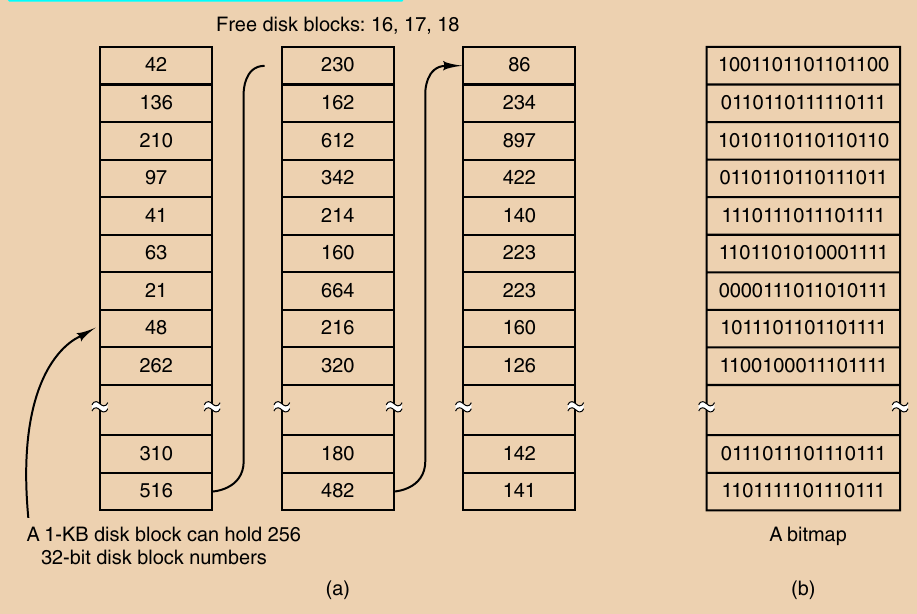
\includegraphics[width=0.45\textwidth]{img/5-18.png}
  \end{center}
  \caption{}
  \label{fig:}
\end{figure}

\subsubsection{Confiabilidade do sistema de arquivos}

A destruição de um sistema de arquivos é muito mais desatrosa do que a destruição de um computador. Se um sistema de arquivos for irrevocavelmente perdido, seja por hardware, software ou ratos nas fitas de backup, restaurar todas as informações será muito difícil e consumirá muito tempo no melhor caso, em muitos será impossível.

Discos rígidos têm blocos ruins desde sua fabricação: é muito caro para o fabricante livrar todos os blocos de defeitos. Uma solução simples de software para blocos ruins existe. Essa solução requer que o usuário ou o sistema de arquivos cuidadosamente contrua um arquivo constituido de todos os blocos ruins. Essa técnica remove eles da lista de blocos livres, para que eles nunca ocorram em arquivos de dados. Se o arquivo de blocos ruins nunca for lido ou escrito, nenhum problema surgirá. Deve-se ter cuidado durante backups para que esse arquivo não seja lido.

\subsubsection{Backups}

A maioria das pessoas não acham que backups valem a pena, até que em um dia tranquilo seus discos morram abruptamente. 

Backups modernos são geralmente feitos em fitas magnéticas, devido a seu baixo custo por giga armazenado. Fazer backups não é tão trivial e alguns cuidados precisam ser tomados.  

Backups são feitos quando é preciso recuperar do desastre ou recuperar da estupidez. O primeiro caso é menos comum e ocorre depois de um crash de disco, incêndio, ou outra catástrofe natural. Na prática, essas coisas não acontecem muito frequentemente e é por isso que muitas pessoas não se preocupam com backups. O segundo motivo é quando usuários acidentalmente removem arquivos importantes. Esse problema acontece tão frequentemte que quando um arquivo é "removido" no Windows, ele não é deletado, apenas movido para um diretório especial, a lixeira.

Fazer um backup demora bastante tempo e ocupa um grande quantidade de espaço, por isso, fazer eficientemente e convenientemente é importante.

O primeiro ponto é analisar quais arquivos do sistema de arquivos devem ser incluidos no backup. Certamente, não é necessário incluir todo o sistema de arquivos. Vários programas executáveis podem ser reinstalados a partir de CD-ROMs ou de arquivos fonte, então não precisam ser incluídos. Arquivos temporários também não. Em sistemas \unix, todos os arquivos especiais (dispositivos de entrada e saída) são mantidos num diretório /dev. Não só incluir esses arquivos no backup é desnecessário como é perigoso, pois o programa de backup pode rodar indefinidamente se tentar ler por completo esses arquivos. 

Segundo, é desnecessário incluir arquivos que não mudaram desde o último backup: \textbf{backups incrementais}. A forma mais simples de fazer backups incrementais é fazer um backup completo periodicamente, e outros menores diariamente incluindo somente arquivos que mudaram desde o último backup completo (ou diário).

Esse esquema incremental dificulta a restauração. Para recuperar um arquivo, primeiro deve ser restaurado o último backup completo seguido dos backups incrementais em ordem reversa.

Outro problema é que, devido a natureza do processo, grandes quantidades de dados estão presentes nos backups e, por isso, alguma compressão pode ser necessária. Até ai tudo bem, o problema surge quando um único "bad spot" na fita pode invalidar um arquivo inteiro ou até mesmo toda a fita. Portanto, o processo de comprimir o backup deve ser tomado com bastante cuidado.

Uma quarta questão a se considerar é a dificuldade de fazer um backup em um sistema de arquivos ativo. Se arquivos estão sendo modificados durante o backup, o backup resultante pode ser inconsistente. Por essa razão, algoritmos foram escritos para fazer snapshots rápidos do sistema de arquivos ao copiar estruturas de dados críticas, e então requerir mudanças futuras dos arquivos para copiar os blocos em vez de atualizá-los in place. Dessa forma, o sistema de arquivos é efetivamente congelado no momento do snapshot, para ser feito um backup "sem pressa".

Por último, fazer backups introduz problemas não técnicos. O melhor sistema de segurança online pode ser inútil se o administrador do sistema deixa todas as fitas de backup em seu escritório e o deixa aberto e desprotegido toda vez que caminha até o corredor para pegar um café, por exemplo. Problemas desses tipo devem ser evitados. 

Duas estratégias podem ser feitas para backups em fitas: um \textbf{\textit{dump} físico} ou um \textbf{\textit{dump} lógico}. A primeira estratégia é simples, ela consiste em começar no bloco 0 do disco, escrever todos os blocos na fita e só parar quando tiver copiado o último. Um programa que implementa esse processo é tão simples que provavelmente pode ser escrito de tal forma que fique 100\% livre de bugs. Mesmo assim, há alguns problemas nessa estratégia. Uma delas é que não há valor em incluir no backup blocos inutilizados. Se o programa de \textit{dumping} consegue ter acesso à lista de blocos livres, ele pode evitar incluir blocos inutilizados. No entanto, pular blocos inutilizados implica em manter de alguma forma o número de cada bloco incluido. Outro problema é incluir blocos ruins. Se todos os blocos ruins são remapeados pelo controlador do disco e são escondidos do SO, sem problemas. Por outro lado, se eles são visíveis e mantidos em alguma lista de blocos ruins, é essencial que o programa de dumping tenha acesso essa informação para que não tente ler nenhum bloco ruim. Resumindo, as vantagens de um dump físico são sua simplicidade e eficiência (basicamente, pode rodar na velocidade do disco). As desvantagens são a incapacidade de pular blocos inutilizados, de fazer dumps incrementais e restaurar arquivos individuais. Por esses motivos, a maioria dos sistemas fazem dumps lógicos.

Um \textbf{dump lógico} começa em um ou mais diretórios específicos e recursivamente inclui todos os arquivos e diretórios encontrados que tenham sido modificados desde uma data base.

Para que seja possível restaurar arquivos individuais, todo informação necessária para recriar o caminho ao arquivo deve ser incluida no backup. Ou seja, alguns diretórios não modificados devem ser incluídos, juntos com todos seus atributos que dão as permissões originais. 

Restaurar um sistema de arquivos a partir de um backup é simples. Para começar, um sistema de arquivos vazio é criado no disco. Então, o último dump completo é restaurado (diretórios primeiro). Depois, esse processo é repetido para o primeiro backup incremental realizado após esse último completo, e depois para o próximo, e assim por diante.

Observe que como a lista de blocos livres não é um arquivo (e sim uma lista ligada de blocos em disco) não é possível restaurá-la. Então, é necessário construí-la manualmente após a restauração do sistema de arquivos. Isso é possível já que o conjunto de blocos livres é o complemento do conjunto de blocos utilizados, e esse último conjunto pode ser obtido inspecionando os arquivos restaurados.


\subsubsection{Consistência do sistema de arquivos}
Muitos sistemas de arquivo leêm blocos, os modificam e escrevem depois. Se o sistema falha antes que TODOS os blocos tenham sido escritos, o sistema de arquivos pode ficar em um estado inconsistente. Esse problema é particularmente crítico quando alguns dos blocos que não foram escritos são blocos de i-nodes, de diretório ou blocos contendo a lista de blocos livres.

A maioria dos computadores tem programas que checam a consistência do sistema de arquivos. Por exemplo, \unix tem o programa \textit{fsck} e o Windows, \textit{chkdsk}. Programas desse tipo podem ser rodados quando o sistema é inicializado, especialmente depois de uma falha. A descrição abaixo refere-se ao funcionamento do programa \textit{fsck}, mas os princípios aqui considerados são gerais para programas desse tipo.

Dois tipos de incosistência são checadas: de blocos e de arquivos. Para checar incosistência de blocos, o programa constrói duas tabelas, cada uma contendo um contador para cada bloco do disco. Todos os contadores são inicializados com 0. Os contadores da primeira tabela guardam quantas vezes o bloco em questão é apontado por um arquivo; os contadores da segunda tabela guardam quantas vezes o bloco está presente na lista de blocos livres (ou no bitmap). O programa varre todos os i-nodes e atualiza os contadores da primeira tabela e varre a lista de blocos livres e atualiza os contadores da segunda tabela. Em seguida, os contadores das duas tabelas são comparados para todos os blocos.

Observe que, se o sistema de arquivos é consistente, cada bloco tem um "1" ou na primeira tabela ou na segunda, conforme a figura {\color{blue}(a)} abaixo. No entanto, pode haver inconsistências. Analisemos alguns tipos. 

{\color{blue} (b): \textbf{Bloco ausente}}

O primeiro tipo é mostrado em (b), em que o bloco 2 não aparece em nenhuma tabela. Isso é reportado como um erro de \textbf{bloco ausente}. Esse é um erro não causa danos ao sistema, porém há desperdiço de espaço de disco. A solução é direta: basta adicionar o bloco à lista de blocos livres. É fácil ver um cenário em que isso pode acontecer:

Um arquivo aponta para os blocos 1 e 2 e é o único arquivo do sistema que aponta para o bloco 2, Não preciso mais de alguns dados e o arquivo deverá diminuir de tamanho, então, por exemplo, o bloco 2 será livrado. Portanto, o i-node do arquivo não conterá mais o endereço do arquivo 2. Além disso, o bloco 2 deve ser adicionado à lista de blocos livres. Se imediatamente depois de escrevermos no bloco do i-node do arquivo (removendo o endereço do bloco 2) o sistema falhar, a lista de blocos não será atualizada e, então, o bloco 2 não estará presente. Isso resulta em um erro de bloco ausente. 

{\color{blue} (c) \textbf{Bloco duplicado na lista de blocos livres}}

O bloco 4 aparece duas vezes na tabela de blocos livre. Duplicatas só podem acontecer em lista ligadas, com bitmap isso é impossível. A solução é simples também: basta reconstruir a lista de blocos livres.



{\color{blue} (d) \textbf{Mesmo bloco em arquivos distintos}}

Esse é o pior cenário possível: o mesmo bloco presente em dois ou mais arquivos. Isso acontece com o bloco 5 na figura. Se algum desses arquivos for removido, o bloco 5 será colocado na lista de blocos livres, levando a uma situação em que o mesmo bloco está em uso e na lista de blocos livres ao mesmo tempo. Se ambos os arquivos forem removidos, o arquivo será adicionado duas vezes na lista de blocos livres. A solução apropriada é alocar um bloco livre, copiar o conteúdo do bloco 5 nele e inserir a copia em algum dos arquivos. Dessa forma, o conteúdo dos dois arquivos fica inalterado (apesar de que certamente algum dos dois contém uma informação estranha), mas o sistema de arquivos fica consistente. O erro deve ser reportado, para que o usuário possa tratá-lo.

\begin{figure}[h]
  \begin{center}
    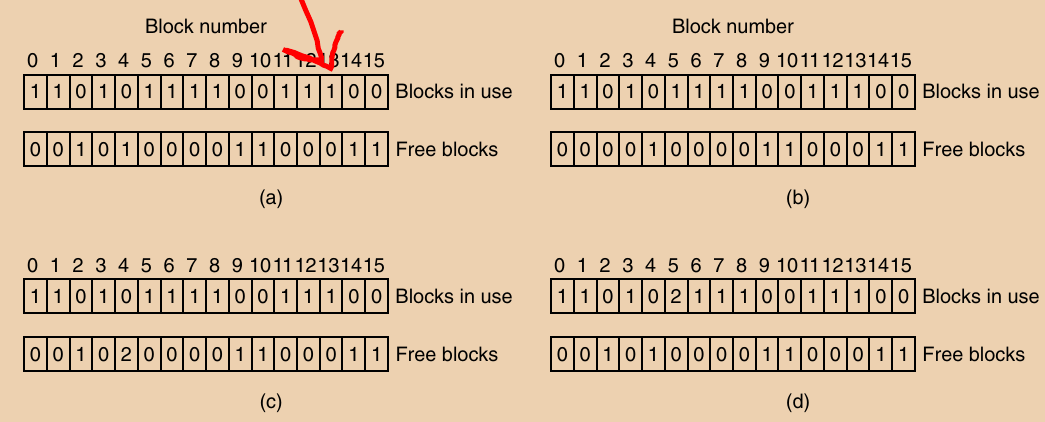
\includegraphics[width=0.6\textwidth]{img/5-19.png}
  \end{center}
  \caption{}
  \label{fig:}
\end{figure}


Outro tipo de checagem é checagem por arquivo. É construida uma tabela que conta, para cada arquivo, a quantidade de vezes que aparece na árvore de arquivos. O contador de cada arquivo é comparado com o número armazenado no i-node. Esses números devem coincidir. Observe que links simbólicos não fazem o contador no i-node aumentar, somente hard links.

Temos dois tipos de inconsistências, quando esses números não concordam.

\begin{itemize}
  \item {\color{blue} Contador no i-node maior que o número de aparições na árvore.}

    Nesse caso, mesmo que todos arquivos sejam excluídos, o contador do i-node será não nulo e, portanto, não será removido. Isso desperdiça espaço de disco.   
  \item {\color{blue} Contador no i-node maior que o número de aparições na árvore.}
  
    Esse erro pode ser catastrófico. De fato, se alguns arquivos são removidos, o contador do i-node pode chegar a 0, e sendo assim, seus blocos serão liberados. Isso fará que o restante dos arquivos que apontavam para esse i-node sejam efetivamente deletados. 
\end{itemize}

A solução é corrigir o valor do contador do i-node.

Outros tipos de checagem são possíveis. Exemplos: 
\begin{itemize}
  \item se o número de um i-node é maior que o número de i-nodes no disco, algo está errado. 
  \item modos incomuns de arquivos em i-nodes, como 0007.
  \item arquivos localizados em diretórios de usuário, porém pertencentes ao super-usuário e com o bit SETUID ativado. Isso gera problemas de segurança visto que tais arquivos podem adquirir poderes de super-usuário quando executados por qualquer usuário.
\end{itemize}

Com um pouco de esforço, é possível pensar em uma lista relativamente longa de situações peculiares (tecnicamente legais) que podem ser reportadas.

Alguns sistemas de arquivos protegem o usuário dele mesmo. Por exemplo, um usuário pode querer excluir todos os arquivos objetos de um diretório e rodar rm * .o em vez de rm *.o (observe o espaço no primeiro comando). Em alguns sistemas, nenhum bloco é retornado à lista de blocos livres até que eles sejam realmente necessários. Isso permite que usuários que perceberem o erro rápido o suficiente, rodem programas de "desremoveção" de arquivos. Mecanismos desse tipo são inseguros. Um sistema seguro deveria escrever lixo nos blocos de dados quando um arquivo é removido, para que outro usuário não consiga recuperar informação.

\subsection{Performance do sistema de arquivos}
O acesso ao disco é muito mais lento que o acesso à memória. Ler um palavra na memória pode demorar 10 nsec. Leituras ao disco podem acontecer a 10 MB/sec, o que é 40 vezes mais devagar por palavra de 32 bits, e isso deve ser adicionado de 5-10 msec referente ao seek. Se uma única palavra é necessária, o acesso à memória é da ordem de 1 milhão de vezes mais rápido que o acesso ao disco. Então, muitos sistemas de arquivos foram escritos com várias otimizações para melhorar o desempenho.

\subsubsection{Cache}

A técnica mais comum usada para reduzir acesso ao disco é o \texttbf{cache de bloco}. Nesse contexto, um cache é uma coleção de blocos que logicamente pertencem ao disco mas são mantidos em memória para melhorar desempenho.

Vários algoritmos podem ser usados para lidar com o cache, mas o mais comum é checar todas as chamadas de \verb|read| para ver se os blocos necessários estão no cache. Caso esteja, não é necessário acessos ao disco. Caso contrário, o bloco é lido do disco para o cache e depois copiada para aonde for pedido. Pedidos subsequentes de leitura do mesmo bloco são feitos usando o bloco no cache.

O jeito usual de verificar se um dado bloco está no cache é usando uma tabela de hash. Quando um bloco é carregado em um cache cheio, algum bloco deve ser movido (e escrito no disco se foi modificado desde que foi movido para o cache) e todos os algoritmos usuais de substituição de páginas de memória podem ser usados. Uma coisa boa diferente entre paginação e o processo de cache de blocos é que referências de cache são relativamente infrequentes, então é factível deixar todos os blocos na ordem LRU (Least Recently Used) exata com listas ligadas.

\begin{figure}[h]
  \begin{center}
    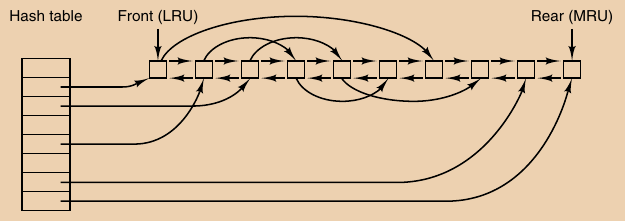
\includegraphics[width=0.45\textwidth]{img/5-20.png}
  \end{center}
  \caption{}
  \label{fig:}
\end{figure}

Acontece que a ordem LRU não é desejada nesse caso. Se um bloco crítico, como um i-node, é trazido ao cache e modificado, mas não escrito ao disco, uma falha pode deixar o sistema num estado incosistente. Se o bloco de i-node for colocado no final da lista LRU, pode demorar um pouco a atingir o começo e ser reescrito no disco.

Além disso, alguns blocos, como blocos de i-nodes, raramente são referenciados duas vezes em um intervalo de tempo curto. Essas considerações levaram a um esquema LRU modificado, levando dois fatores em consideração:
\begin{itemize}
  \item É provável que o bloco seja requerido denovo em breve?
  \item O bloco é essencial para a consistência do sistema de arquivos?
\end{itemize}

Blocos que provavelmente não serão requisitados em breves são colocados no começo, então, seus buffers serão usados rapidamente. Já os blocos que devem ser requisitados são colocados no final, e ficarão um tempinho por ali.

A segunda questão é independente da primeira. Se um bloco é essencial para a consistência (basicamente, tudo menos dados) e foi modificado, ele deve ser escrito no disco imediatamente, independente de sua posição na lista LRU. Isso reduz o risco de uma falha quebrar o sistema de arquivos.

Mesmo assim, não é desejável manter dados de blocos na cache por muito tempo antes de escrevê-los em disco. Considere um escritor escrevendo um livro num editor de texto. Mesmo que periodicamente o escritor diga ao editor para escrever o arquivo sendo editado no disco, há uma boa chance de tudo ainda estar no cache e nada no disco. Se o sistema falhar, a estrutura do sistema de arquivos não será corrompida, mas o dia de trabalho do escritor será desperdiçado. 

No \unix, há uma chamada de sistema, \verb|sync| que força todos blocos modificados a serem escritos em disco imediatamente. Quando o sistema é inicializado, um programa, geralmente chamado \textit{update}, é executado em segundo plano. Ele tem um loop infinito requerindo chamadas \verb|sync| e dormindo por 30 segundos entre chamadas. Como resultado, não mais que 30 segundos de trabalho são perdidos devido a falhas do sistema.

O jeito Windows é escrever todo bloco modificado imediatamente. Caches em que todos os blocos modificados são escritos no disco imediatamente são chamados de \textbf{caches write-through}. A diferença desses métodos pode ser exemplificada da seguinte forma. Suponha que queremos escrever um bloco de 1-KB, um caractere de cada vez. \unix irá coletar todos os caracteres no cache e escrever o bloco a cada 30 segundos, ou toda vez que o bloco é removido do cache (cache \textbf{write-back}). O Windows vai fazer um acesso ao disco a cada caractere escrito. Evidentemente, a maioria dos programas fazem um buffering interno, então normalmente eles não escrevem um caractere e sim uma linha inteira ou uma unidade maior a cada chamada \verb|write|.

Outro ponto relacionado a estratégias de caches é a decisão de alocar um bloco de cache ou não quando temos um cache miss na escrita. Geralmente, é usado write-back com write-allocation (com esperança de futuras escritas no mesmo bloco) e write-through sem write-allocation (como o bloco é escrito imediatamente, não há vantagens em colocá-lo no cache para futuras escritas). 

\begin{figure}[h]
  \begin{center}
    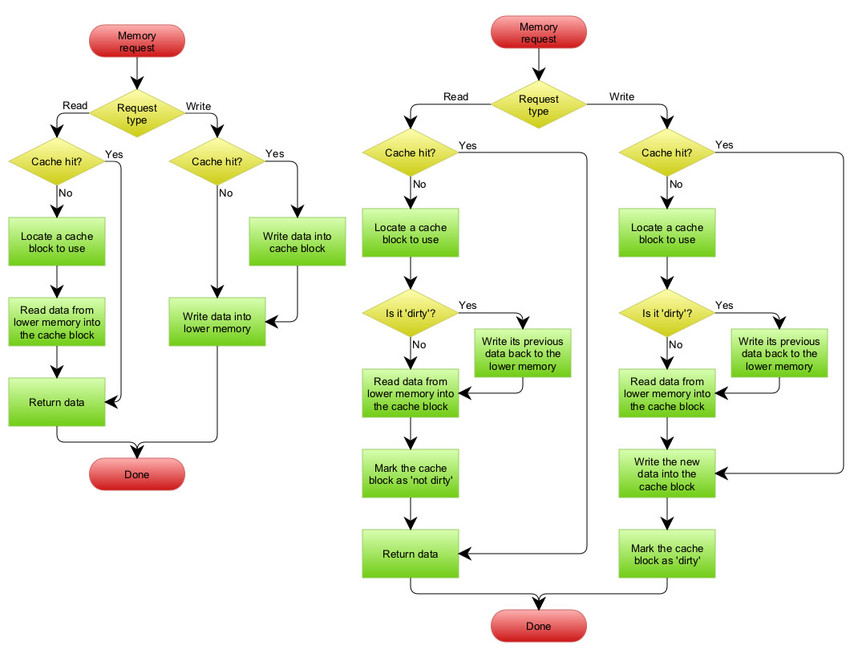
\includegraphics[width=0.73\textwidth]{img/cache.jpg}
  \end{center}
  \caption{}
  \label{fig:}
\end{figure}

\newpage

Uma consequência dessa diferença de estratégias de caching (\textbf{write-back} e \textbf{write-through}) é que remover um disco floppy de um sistema \unix sem ffazer uma \verb|sync| provavelmente resultará em dados perdidos e frequentemte um sistema de arquivos corrompido. No Windows, isso não acontece. Essas diferentes estratégias foram escolhidas porque o \unix foi desenvolvido num ambiente onde quase todos os discos eram discos rígidos, enquanto o Windows foi desenvolvido num ambiente de discos floppy. A medida que discos rígidos viraram regra, o método \unix, com sua melhor eficiência, virou regra e é hoje também utilizado pelo Windows para discos rígidos.

\subsubsection{Prefetch}

A segunda técnica para melhorar o desempenho do sistema de arquivo é tentar colocar blocos no cache antes deles serem requisitados para aumentar a taxa de cache hit.

Certamente, essa estratégia de \textbf{prefetch} só funciona bem se o arquivo está sendo lido sequencialmente. Se o arquivo está lendo aleatoriamente, isso na verdade é prejudicial pois blocos desnecessários são lidos e substituem potenciais blocos úteis no cache.

Para decidir se vale a pena fazer prefetch, o sistema de arquivos pode manter padrões de acessos para os arquivos. Inicialmente, o arquivo é dado o "benefício da dúvida" e é colocado no modo "acesso sequencial". No entanto, sempre que um seek é feito, esse bit é desativado. Se leituras sequenciais são feitas posteriormente, o bit é ativado novamente.

\subsubsection{Reduzindo Movimentos de braço de disco}

Outra forma importante de otimização é a redução de movimento do braço do disco ao colocar blocos que são prováveis de ser acessados em sequência próximos entre si, preferencialmente no mesmo cilindro.

Quando um arquivo de saída é escrito, o sistema de arquivos deve alocar os blocos um de cada vez, a medida que são necessários. Se os blocos livres são mantidos num bitmap, e todo o bitmap está em memória, é suficientemente fácil escolher um bloco livre mais perto possível do bloco anterior. Com uma lista ligada, na qual parte está no disco, isso é bem mais difícil. Mesmo assim, é possível.

(verificar essa parte no livro traduzido, não entendi totalmente)

O truque é manter o uso de disco não em blocos e sim em grupos de blocos consecutivos. Se setores consistem em 512 bytes, o sistema poderia usar blocos de 1-KB (2 setores) mas alocar espaço em disco em unidades de dois blocos (4 setores). Isso não é o mesmo que ter blocos de 2-KB, já que o cache continuaria usando blocos de 1-KB e as transferências de disco continuariam 1-KB, mas ler um arquivo sequencialmente num sistema ocioso reduziria o número de seeks por um fator de dois, o que é uma melhoria considerável.

Outro gargalo em sistemas que usa algo parecido com i-nodes é que as leituras em arquivos pequenos requer dois acessos: um para o i-node e outro para o bloco. Todos os i-nodes estão perto do começo do disco, confrme a figura abaixo. Então, a distância média entre um i-node e seus blocos é aproximadamente metade do número de cilindros, o que requer seeks longos.

\begin{figure}[h]
  \begin{center}
    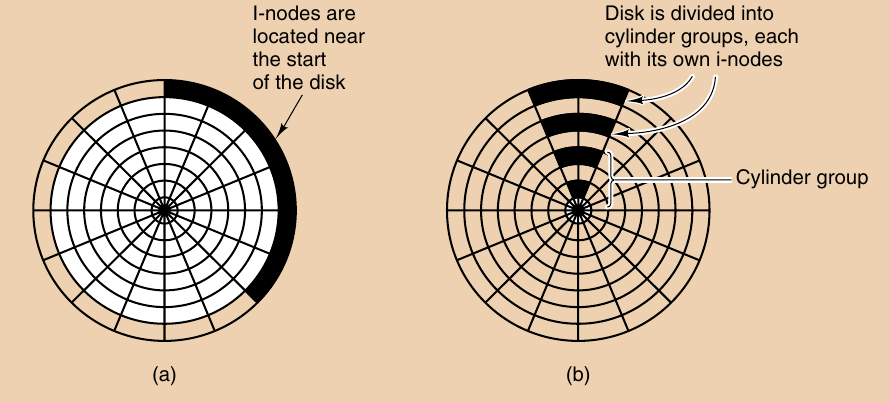
\includegraphics[width=0.6\textwidth]{img/5-21.png}
  \end{center}
  \caption{}
  \label{fig:}
\end{figure}

Uma melhoria fácil é colocar os i-nodes no meio do disco, em vez do começo. Isso reduz o seek médio pela metade. Outra ideia, mostrada em (b), é dividir o disco em grupos de cilindros, cada um com seus próprios i-nodes, blocos e lista de blocos livres. Quando se cria um arquivo, qualquer i-node pode ser escolhido, mas é feita uma tentativa de achar um bloco no mesmo grupo de cilindro do i-node. Se nenhum estiver disponível, então um bloco em um cilindro próximo é usado.

\newpage

\subsection{Sistema de arquivos estruturado em log}

Mudanças na tecnologia estão colocando pressão nos sitemas operacionais atuais. Em particular, CPUs estão ficando mais rápidas e as memórias crescendo exponencialmente. Enquanto isso, o tempo de seek em disco está estagnado. Devido a esse gargalo, pesquisas feitas em Berkley tentaram aliviar esse problema ao construir um novo tipo de sistemas de arquivos, o \textbf{LFS (Log-structured File System)}. Descrevemos como esse sistema funciona.

Por causa dos avanços citados acima, caches de disco estão crescendo rapidamente. Consequentemente, é possível satisfazer uma fração substencial de todos os pedidos de leitura direto do cache, sem precisar acessar o disco. Por essa observação, a maioria dos acessos aos discos serão de escrita, no futuro. Então, o uso do mecanismo de prefetch não aumentará muito o desempenho.

Além disso, vale ressaltar que a maioria das escritas em discos são feitas em pequenos arquivos. Escritas em arquivos pequenos são extremamente ineficientes, já que uma escrita de 50$\mu$sec geralmente é precedida por um seek de 10-msec e um delay rotacional de 4-msec. Um exemplo de escrita comum em um arquivo pequeno é a criação de um novo arquivo num sistema \unix. Para escrever esse arquivo, o i-node do diretório, o bloco do diretório, o i-node do arquivo e o próprio arquivo precisam todos ser escritos. É verdade que essas escritas podem ser "deixadas pra depois", mas isso expõe o sistema a problemas de inconsistência. Por essa razão, escritas em i-nodes são feitas, de forma geral, imediatamente.

A ideia básica é estruturar o arquivo como um log. Periodicamente, e também quando há uma necessidade especial, todos as escritas pendentes que estão no buffer da memória são coletadas num único segmento e escritas no disco como um único segmento contíguo no final do log. Um único segmento pode conter, então, i-nodes, blocos de diretório, bloco de dados e outros tipos de blocos todos misturados. No começo de cada segmento há um sumário do segmento, dizendo o que pode ser encontrado no segmento. Se o segmento médio pode ser feito com tamanho aproximadamente 1 MB, quase todo o disco pode ser utilizado.

Nesse design, i-nodes podem continuar existindo e tem a mesma estrutura que no \unix, mas agora eles estão espalhados por todo o log, em vez de estarem numa posição fixa no disco. Mesmo assim, quando um i-node é localizado, localizar os blocos é feito da maneira usual. Evidentemente, localizar i-nodes agora é mais difícil, já que seu endereço não pode ser calculado pelo seu número, como no \unix. Para ser possível localizar i-nodes, é preciso um mapa de i-nodes. O mapa é mantido no disco, mas as partes mais usadas podem ser colocadas na memória para aumentar o desempenho.

Se os discos fossem infinitamente grandes, a descrição acima seria a história completa. No entanto, discos são finitos e o log poderá eventualmente ocupar todo o disco. Felizmente, muitos segmentos contêm blocos que não são mais necessários.

Para lidar com isso, o LFS tem um \textbf{cleaner} que tem a função de escanear o log circularmente para compactá-lo. Ele procura por blocos em desuso nos segmentos. Caso haja "dados vivos", eles vão para a memória e são reescritos num próximo segmento. Os segmentos livrados são marcados, para que o log possa usá-los para novos dados.

Em resumo, o disco é um grande buffer circular, com a thread de escrita adicionando novos segmentos no início e o cleaner removendo antigos de trás.

Perceba que essa técnica de manter arquivos no sistema não é trivial. Quando um bloco de um arquivo é escrito de volta em algum novo segmento, o i-node do arquivo, que está em algum lugar do log, deve ser encontrado e atualizado, e colocado na memória para ser escrito no próximo segmento. O mapa de i-nodes também deve ser atualizado para apontar para a nova entrada. Apesar dessa complexidade, os resultados de desempenho mostram que esse esquema vale a pena. Medidadas feitas no artigo publicado (https://people.eecs.berkeley.edu/~brewer/cs262/LFS.pdf) mostram que o LFS supera o unix em uma ordem de magnitude em escritas pequenas, enquanto tem desempenho semelhante para escritas grandes.





\end{document}




